% D.17 菱形 ABCD，AC=8，BD=6
\documentclass[tikz,border=4pt]{standalone}
\usepackage{ctex}
\usepackage{amsmath}
\usetikzlibrary{calc}
\begin{document}
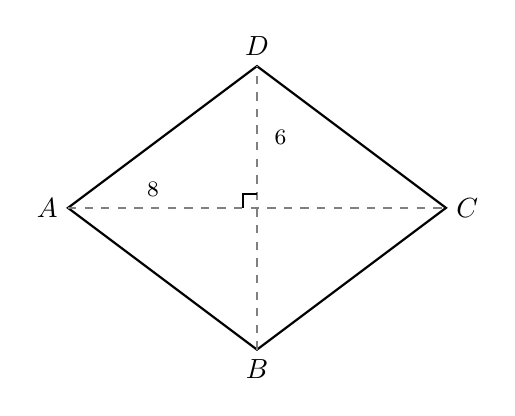
\begin{tikzpicture}[scale=0.6, thick]
  \coordinate (A) at (-4, 0);
  \coordinate (B) at ( 0,-3);
  \coordinate (C) at ( 4, 0);
  \coordinate (D) at ( 0, 3);

  \draw (A) -- (B) -- (C) -- (D) -- cycle;
  \draw[gray, dashed] (A) -- (C);
  \draw[gray, dashed] (B) -- (D);
  % 直角符号 at center
  \draw (-0.3,0) -- (-0.3,0.3) -- (0,0.3);

  \node[left]  at (A) {$A$};
  \node[below] at (B) {$B$};
  \node[right] at (C) {$C$};
  \node[above] at (D) {$D$};
  \node at (-2.2, 0.4) {\footnotesize $8$};
  \node at ( 0.5, 1.5) {\footnotesize $6$};
\end{tikzpicture}
\end{document}
